% Este trabalho está licenciado sob a licença Creative Commons CC-BY-SA.
% Você é livre para usar, compartilhar e adaptar este material, desde que seja atribuída a autoria e que as obras derivadas mantenham a mesma licença.

%--------------------ELEMENTOS PRÉ-TEXTUAIS--------------------%

%-----------------------------Capa-----------------------------%
\imprimircapa

%------------------------Folha de rosto------------------------%
\imprimirfolhaderosto


%----------------------Ficha Catalográfica----------------------%

\begin{fichacatalografica}
    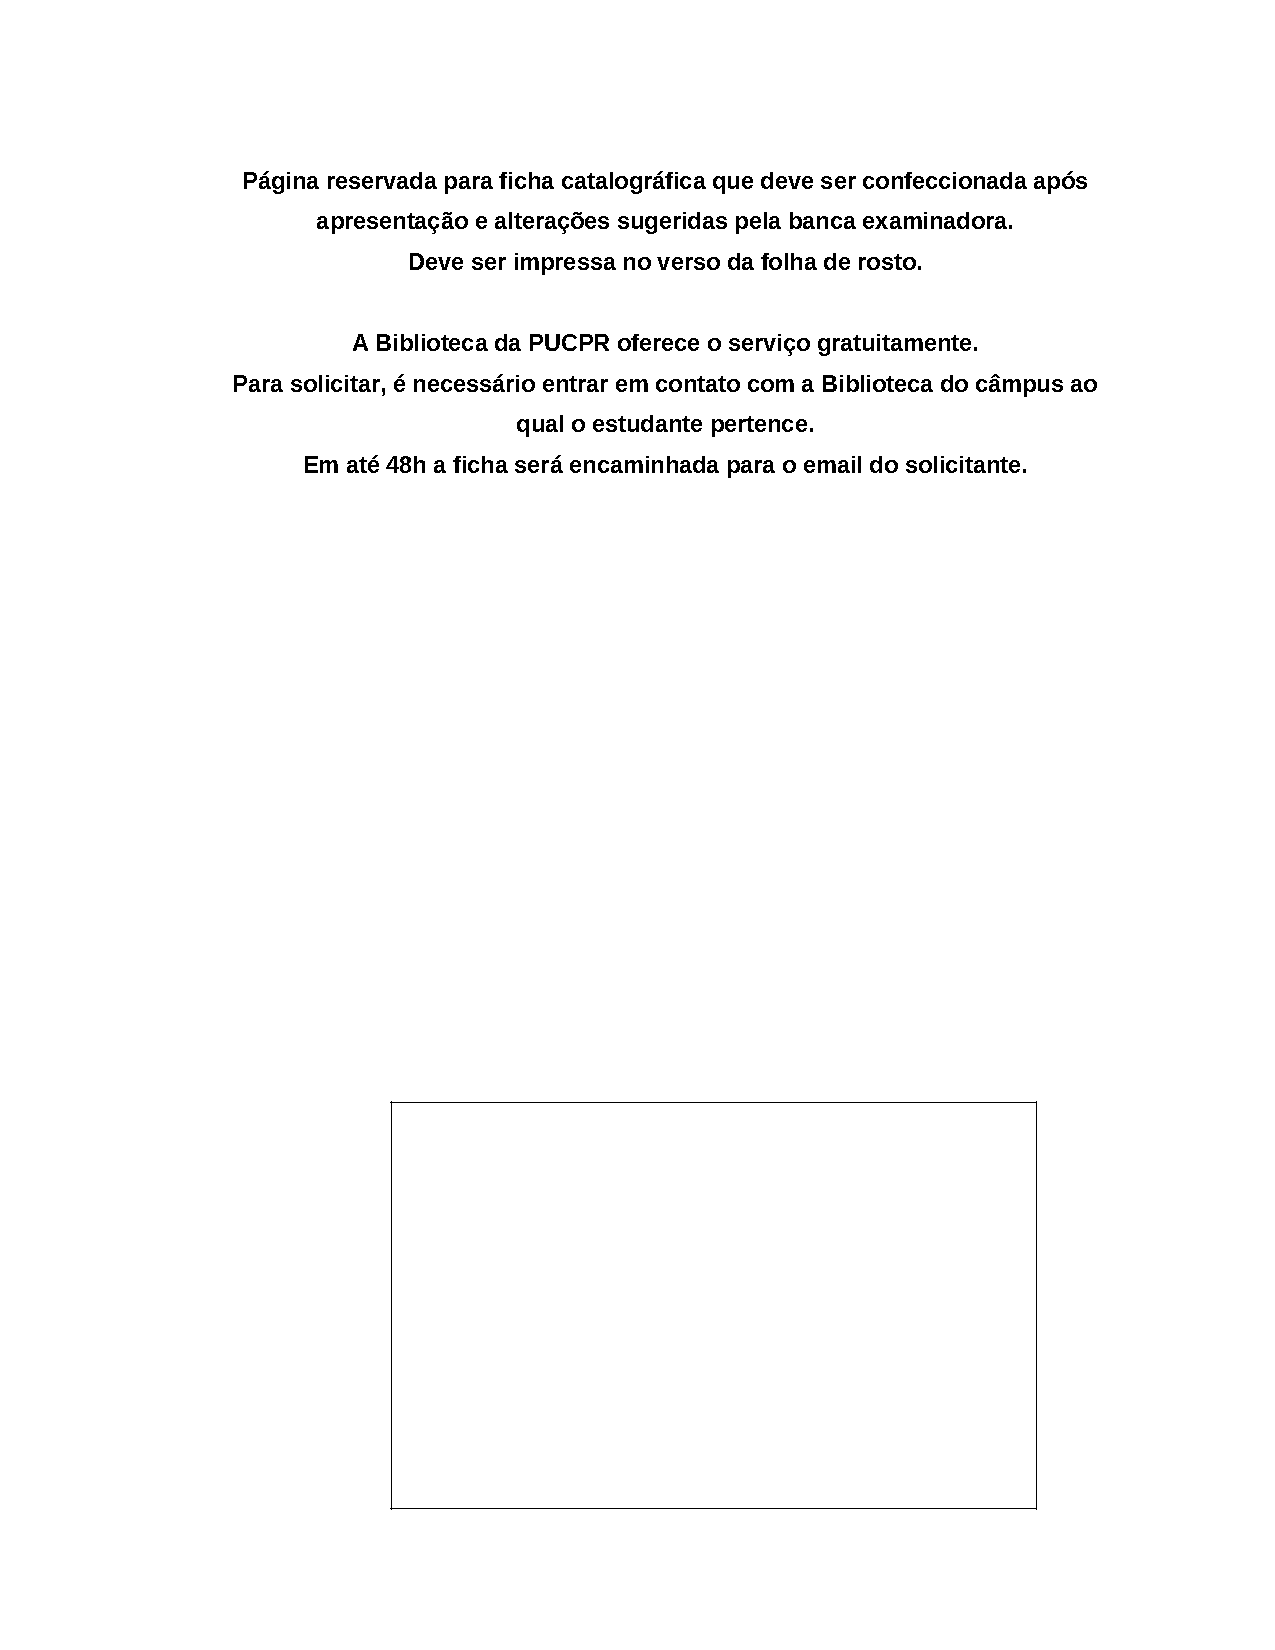
\includepdf{pdfs/ficha_catalografica.pdf}
\end{fichacatalografica}

%----------------------Folha de Aprovação----------------------%

% Após aprovação do trabalho, solicite do orientador a Folha de Aprovação assinada pela Banca Examinadora.
% Salve-a em formato PDF com o nome: folha_aprovacao.pdf
% Substitua o arquivo temporário de mesmo nome presente neste modelo.

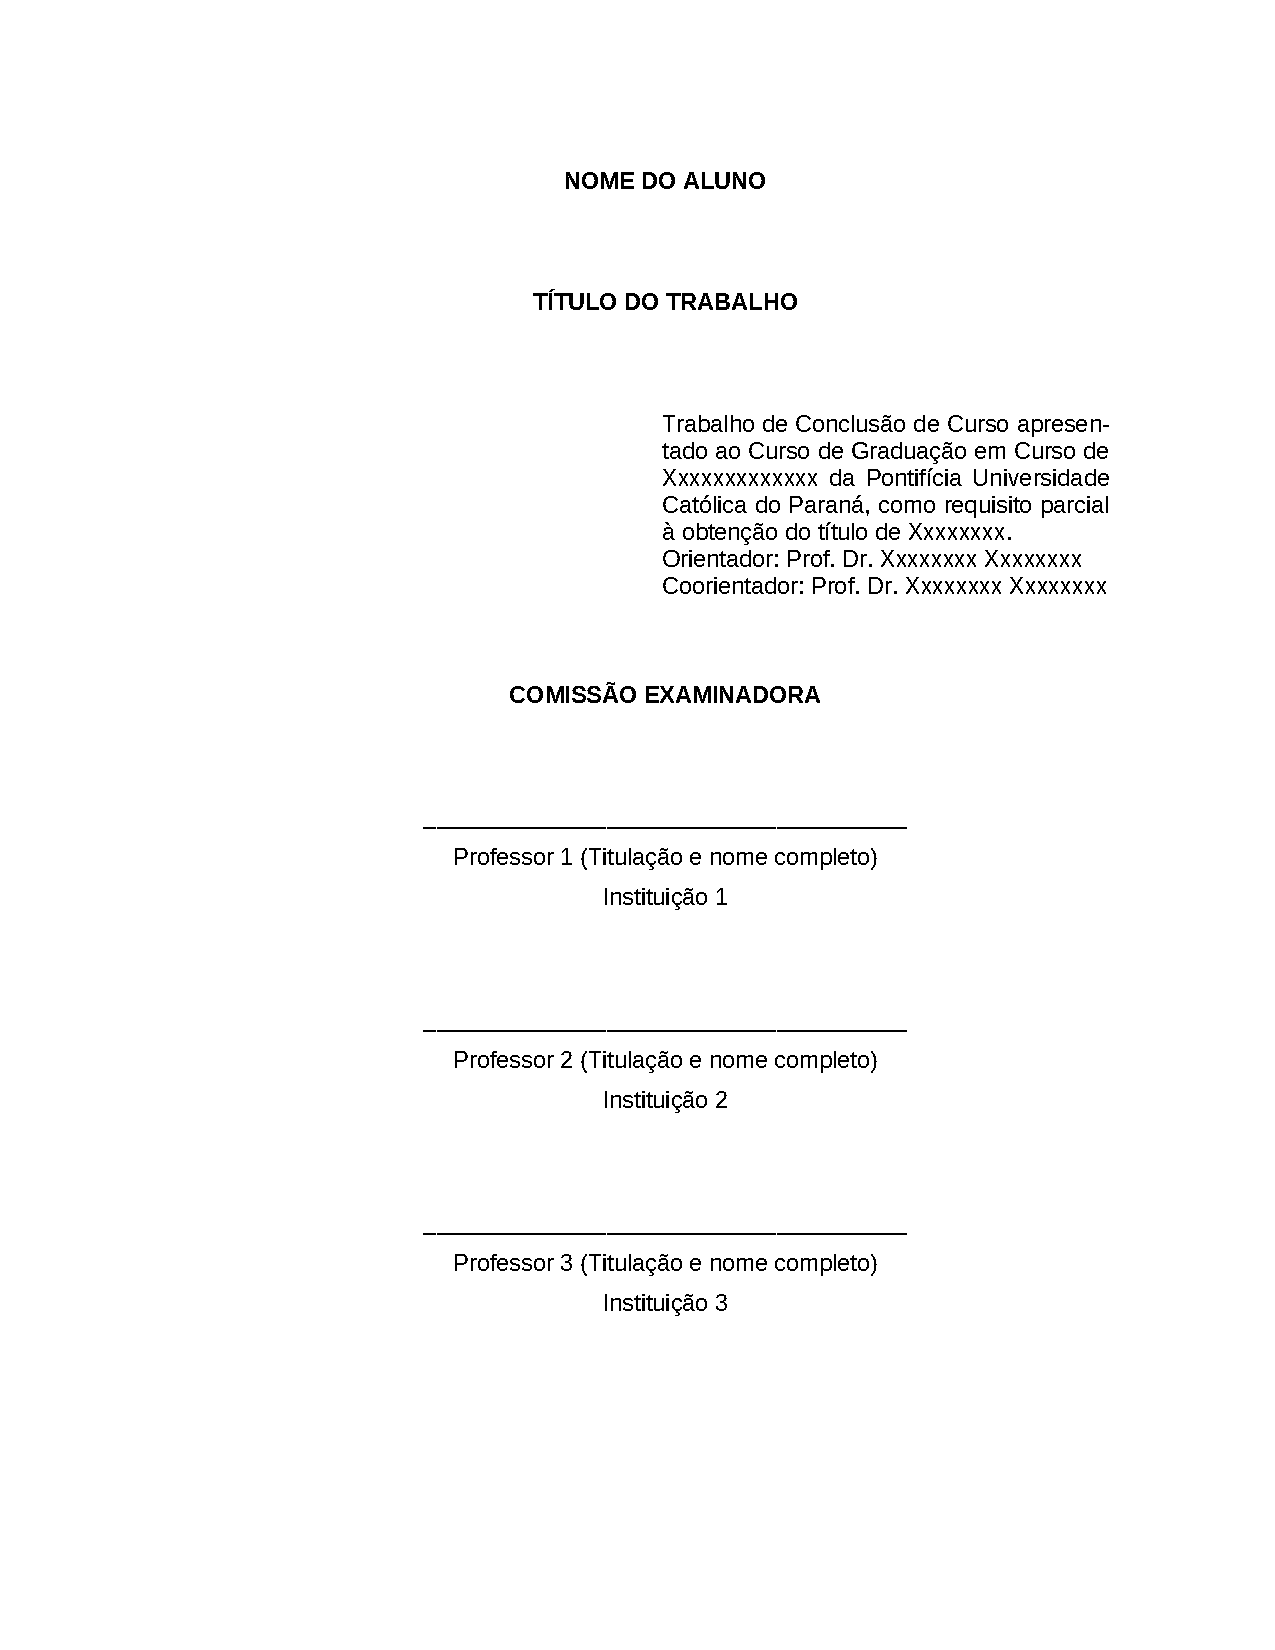
\includepdf{pdfs/folha_aprovacao.pdf}


%----------------------Dedicatória----------------------%
\begin{dedicatoria}
\vspace*{\fill}
\begin{flushright}
\begin{minipage}{8.5cm}
\raggedleft
\textit{
A dedicatória teste Joyce agora
}
\end{minipage}
\end{flushright}
\end{dedicatoria}



%----------------------Agradecimentos----------------------%
\begin{agradecimentos}


Agradeço à Pontifícia Universidade Católica do Paraná...

Agradeço também ao órgão de fomento XYZ...  

Sou grato(a) ao(à) meu(minha) orientador(a)... 

Por fim, mas não menos importante, agradeço aos familiares e amigos...

\end{agradecimentos}




%----------------------Epígrafe----------------------%
\begin{epigrafe}
    \vspace*{\fill}
    \begin{flushright}
        \begin{minipage}{8.5cm}
            \raggedleft
            \textit{
                A epígrafe é a frase de um autor cujo tema tenha relação com o trabalho.\\Não é obrigatório constar na lista de referências a citação da epígrafe.\\[\baselineskip]
                (Autor)
            }
        \end{minipage}
    \end{flushright}
\end{epigrafe}


%----------------------Resumos----------------------%
%----------------Resumo em Português----------------%
\begin{resumo}
\SingleSpacing

    \noindent O texto do resumo convém ter entre 150 e 500 palavras. O texto do resumo deve conter a apresentação do tema, o problema ou objetivo geral da pesquisa, a metodologia e os principais resultados. Deve ser redigido em parágrafo único, na mesma fonte do trabalho e com espaçamento de linhas simples. O texto do resumo convém ter entre 150 e 500 palavras. O texto do resumo deve conter a apresentação do tema, o problema ou objetivo geral da pesquisa, a metodologia e os principais resultados. Deve ser redigido em parágrafo único, na mesma fonte do trabalho e com espaçamento de linhas simples. O texto do resumo convém ter entre 150 e 500 palavras. O texto do resumo deve conter a apresentação do tema, o problema ou objetivo geral da pesquisa, a metodologia e os principais resultados. Deve ser redigido em parágrafo único, na mesma fonte do trabalho e com espaçamento de linhas simples.
    
    \vspace{\onelineskip}
    
    \noindent
    \textbf{Palavras-chave}: palavra 1; palavra 2; palavra 3; palavra 4.
    
\end{resumo}

%----------------Resumo em Inglês----------------%
\begin{resumo}[\textbf{Abstract}]
\SingleSpacing
    \begin{otherlanguage*}{english}
    
        \noindent O texto do resumo em língua portuguesa deve estar traduzido em outra língua (inglês ou francês e/ou espanhol). Abstract abstract abstract abstract abstract abstract abstract abstract abstract abstract abstract abstract abstract abstract abstract abstract abstract abstract abstract abstract abstract abstract abstract abstract abstract abstract abstract abstract abstract abstract abstract abstract abstract abstract abstract abstract abstract abstract abstract abstract abstract abstract abstract abstract abstract abstract abstract abstract abstract abstract abstract abstract abstract abstract abstract abstract abstract abstract abstract abstract.
        
        \vspace{\onelineskip}
        
        \noindent 
        \textbf{Keywords}: keyword 1; keyword 2; keyword 3.
        
    \end{otherlanguage*}
\end{resumo}






%----------------Lista de Ilustrações----------------%
\pdfbookmark[0]{\listfigurename}{lof}
\listoffigures*
\cleardoublepage


%----------------Lista de Quadros----------------%
\pdfbookmark[0]{\listofquadrosname}{loq}
\listofquadros*
\cleardoublepage




%----------------Lista de Tabelas----------------%
\pdfbookmark[0]{\listtablename}{lot}
\listoftables*
\cleardoublepage

%----------------Lista de Gráficos ----------------%
\pdfbookmark[0]{\listplotname}{lop}
\listofplots*
\cleardoublepage


%--------Lista de abreviaturas e siglas---------%
\begin{siglas}
    \item[ABNT] Associação Brasileira de Normas Técnicas
    \item[IBGE] Instituto Brasileiro de Geografia e Estatística
    \item[ISBN] \textit{International Standard Book Number}
    \item[NBR] Norma Brasileira Regulamentar
    \item[PUCPR] Pontifícia Universidade Católica do Paraná
\end{siglas}


%----------------Lista de Símbolos----------------%
\begin{simbolos}
  \item[$ \mathbb{R} $] Conjunto dos números reais
  \item[$ \sum $] Somatório
  \item[$ \dfrac{df}{dx} $] Derivada da função de uma variável $f(x)$ com reação à variável $x$
  \item[$ \overrightarrow{v} $] Vetor
\end{simbolos}


%----------------SUMÁRIO----------------%
\pdfbookmark[0]{\contentsname}{toc}
\tableofcontents*
\cleardoublepage